\documentclass[hyperref,]{ctexart}
\usepackage{lmodern}
\usepackage{amssymb,amsmath}
\usepackage{ifxetex,ifluatex}
\usepackage{fixltx2e} % provides \textsubscript
\ifnum 0\ifxetex 1\fi\ifluatex 1\fi=0 % if pdftex
  \usepackage[T1]{fontenc}
  \usepackage[utf8]{inputenc}
\else % if luatex or xelatex
  \ifxetex
    \usepackage{xltxtra,xunicode}
  \else
    \usepackage{fontspec}
  \fi
  \defaultfontfeatures{Mapping=tex-text,Scale=MatchLowercase}
  \newcommand{\euro}{€}
\fi
% use upquote if available, for straight quotes in verbatim environments
\IfFileExists{upquote.sty}{\usepackage{upquote}}{}
% use microtype if available
\IfFileExists{microtype.sty}{%
\usepackage{microtype}
\UseMicrotypeSet[protrusion]{basicmath} % disable protrusion for tt fonts
}{}
\ifxetex
  \usepackage[setpagesize=false, % page size defined by xetex
              unicode=false, % unicode breaks when used with xetex
              xetex]{hyperref}
\else
  \usepackage[unicode=true]{hyperref}
\fi
\usepackage[usenames,dvipsnames]{color}
\hypersetup{breaklinks=true,
            bookmarks=true,
            pdfauthor={蓝海; 彭莉},
            pdftitle={分析洪流-技术报告},
            colorlinks=true,
            citecolor=blue,
            urlcolor=blue,
            linkcolor=magenta,
            pdfborder={0 0 0}}
\urlstyle{same}  % don't use monospace font for urls
\usepackage{longtable,booktabs}
\usepackage{graphicx,grffile}
\makeatletter
\def\maxwidth{\ifdim\Gin@nat@width>\linewidth\linewidth\else\Gin@nat@width\fi}
\def\maxheight{\ifdim\Gin@nat@height>\textheight\textheight\else\Gin@nat@height\fi}
\makeatother
% Scale images if necessary, so that they will not overflow the page
% margins by default, and it is still possible to overwrite the defaults
% using explicit options in \includegraphics[width, height, ...]{}
\setkeys{Gin}{width=\maxwidth,height=\maxheight,keepaspectratio}
\setlength{\emergencystretch}{3em}  % prevent overfull lines
\providecommand{\tightlist}{%
  \setlength{\itemsep}{0pt}\setlength{\parskip}{0pt}}
\setcounter{secnumdepth}{5}

\title{分析洪流-技术报告}
\author{蓝海 \and 彭莉}
\date{}

% Redefines (sub)paragraphs to behave more like sections
\ifx\paragraph\undefined\else
\let\oldparagraph\paragraph
\renewcommand{\paragraph}[1]{\oldparagraph{#1}\mbox{}}
\fi
\ifx\subparagraph\undefined\else
\let\oldsubparagraph\subparagraph
\renewcommand{\subparagraph}[1]{\oldsubparagraph{#1}\mbox{}}
\fi

\begin{document}
\maketitle

{
\setcounter{tocdepth}{2}
\tableofcontents
}
\section{业绩表现}

\subsection{洪流}

上海财经大学金融学硕士,现任圆信永丰基金管理有限公司首席投资官。历任新疆金新信托证券管理总部信息研究部经理,德恒证券信息研究部副总经理,德恒证券经纪业务管理总部副总经理,兴业证券股份有限公司理财服务中心首席理财分析师,兴业证券股份有限公司上海资产管理分公司副总监。

洪流有丰富的资管经验,在公墓基金方面共管理4个不同的基金产品,其中有增强性债券基金和创设不足一年的混合型基金,我们不做为分析的样本。本文采用的样本是:圆信永丰双红利A和圆信永丰优加生活。

\subsection{当前表现}

\subsubsection{圆信永丰双红利A}\label{a}

\begin{figure}[htbp]
\centering
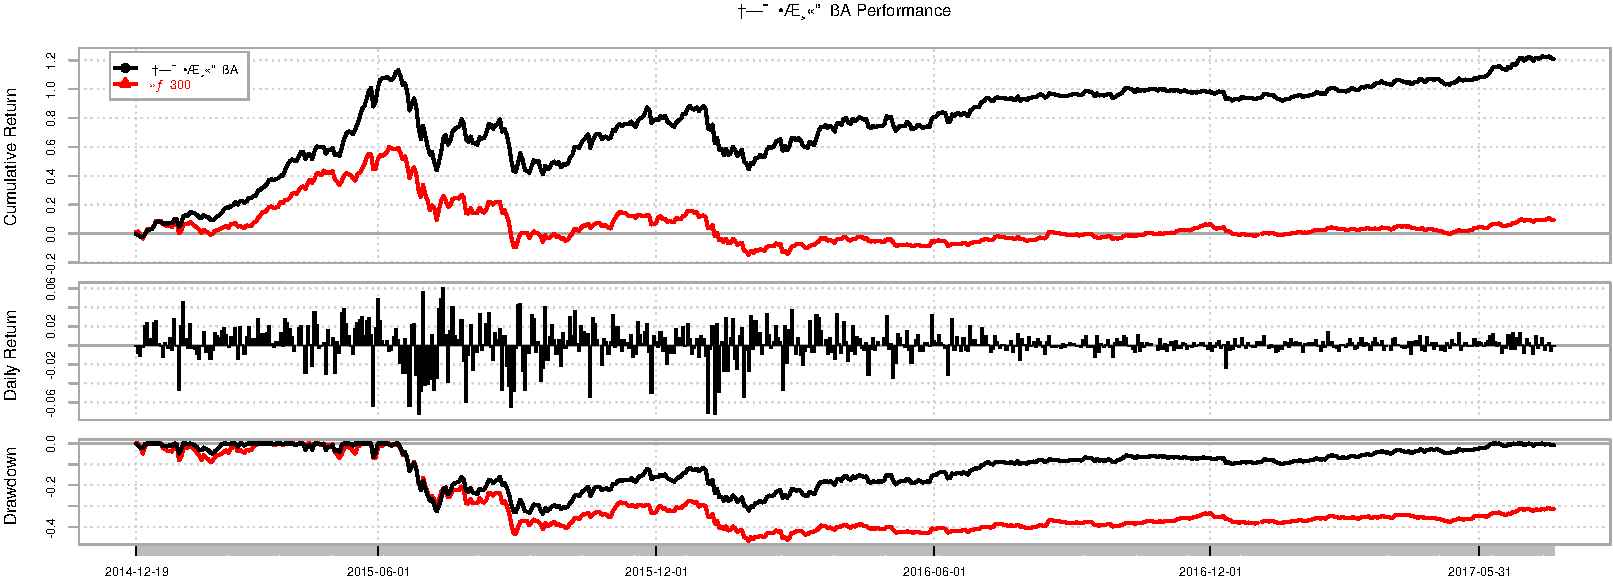
\includegraphics{hongliu-details_files/figure-latex/unnamed-chunk-2-1.pdf}
\caption{基金累计回报率与回撤}
\end{figure}

\begin{longtable}[]{@{}llclclclc@{}}
\toprule
名称 & 近半年 & 夏普率 & 近一年 & 夏普率 & 两年 & 夏普率 & 三年 &
夏普率\tabularnewline
\midrule
\endhead
圆信永丰双红利A & 12.3\% & 2.6 & 18\% & 1.5 & 8.3\% & 0.05 & 121\% &
1.18\tabularnewline
沪深300 & 8.9\% & 1.6 & 16\% & 1.2 & -28.6\% & -0.62 & 14\% &
0.05\tabularnewline
\bottomrule
\end{longtable}

\begin{figure}[htbp]
\centering
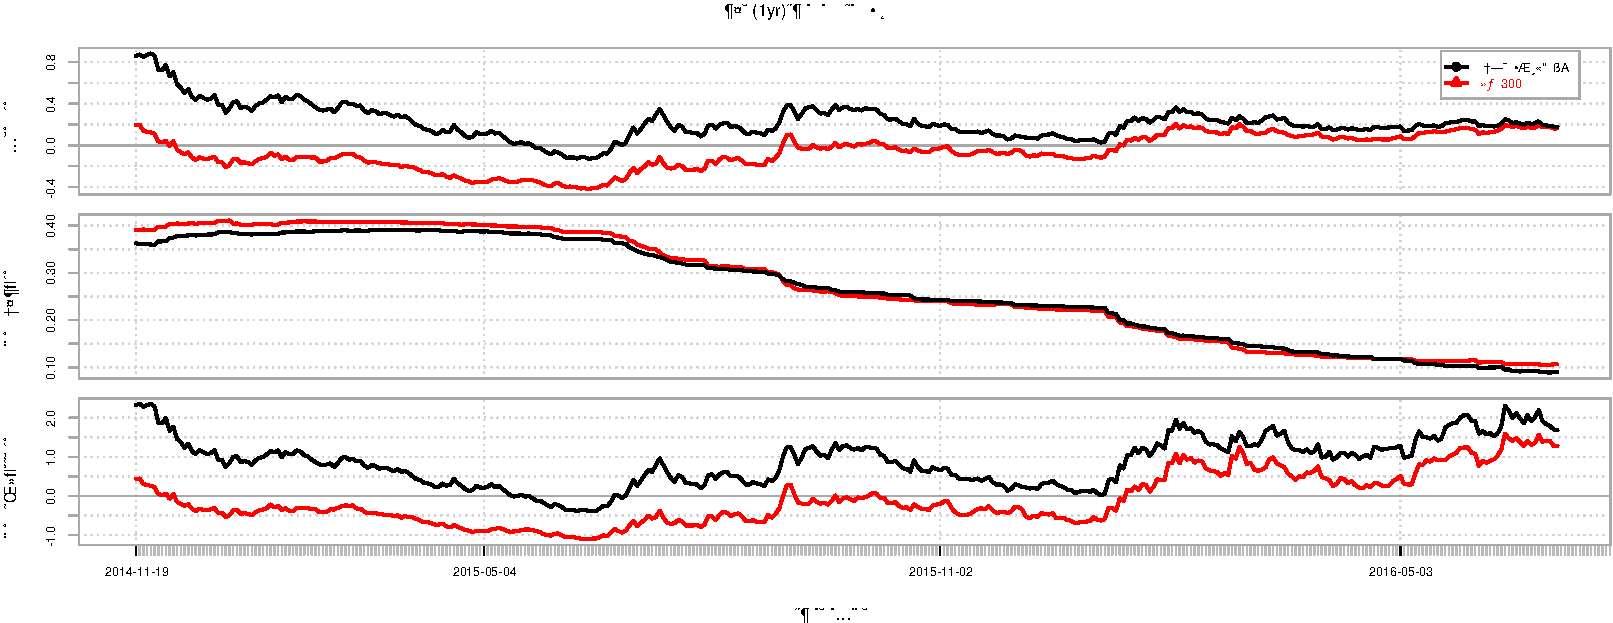
\includegraphics{hongliu-details_files/figure-latex/unnamed-chunk-3-1.pdf}
\caption{投资者收益风险比较}
\end{figure}

图1清楚的表明自洪流在管理该支基金以来相对于沪深300其累计收益率的不俗表现,尤其是在2015年股灾期间,除了第一次大跌外,在股市二次三次探底的过程中,圆信永丰双红利A都较好的控制住了回撤。图2明确的表明,固定一年期的投资者,无论何时买入这两只基金,她都可以获得相比沪深300更高的累计收益,而且面临的波动与沪深300基本相当。因此日收益序列的风险收益比------夏普率------显著高于沪深300。通俗的说,就是不但能够赚更多的钱,而且作为投资者,你还更有可能``拿得住''这样的投资对象,因为收益波动比更大。当然也要注意到该基金的一年期投资收益越来越接近沪深300。

\subsubsection{圆信永丰优加生活}

\begin{figure}[htbp]
\centering
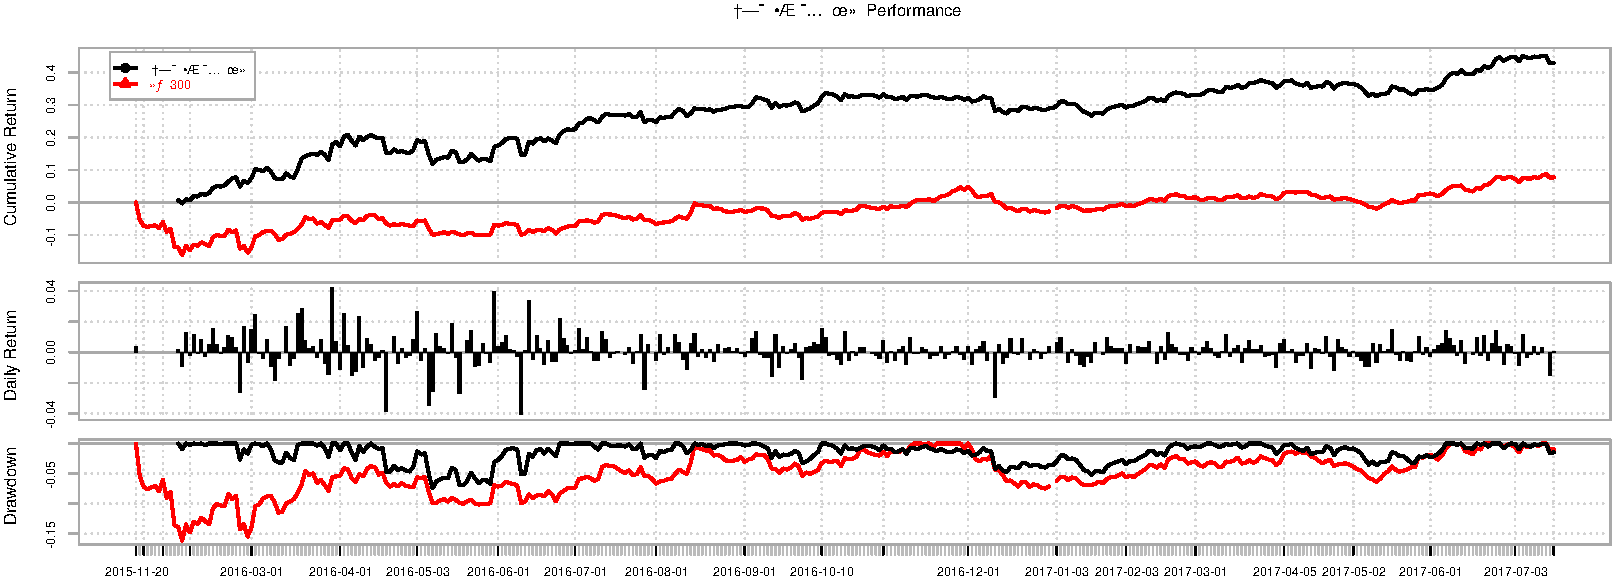
\includegraphics{hongliu-details_files/figure-latex/unnamed-chunk-4-1.pdf}
\caption{基金累计回报率与回撤}
\end{figure}

\begin{longtable}[]{@{}llclclc@{}}
\toprule
名称 & 近半年 & 夏普率 & 近一年 & 夏普率 & 近两年 &
夏普率\tabularnewline
\midrule
\endhead
圆信永丰优加生活 & 9.1\% & 1.6 & 17\% & 1.69 & 43\% &
1.58\tabularnewline
沪深300 & 8.9\% & 1.6 & 16\% & 0.26 & 11\% & 0.18\tabularnewline
\bottomrule
\end{longtable}

这支基金最当引起注意的是回撤控制的力度,整个基金的累计收益率几乎像是缓步爬山一样的一个阶段一个阶段的稳定向上。同期虽然相比沪深300超额收益不大,但是风险少了许多,获取了很高的夏普率。
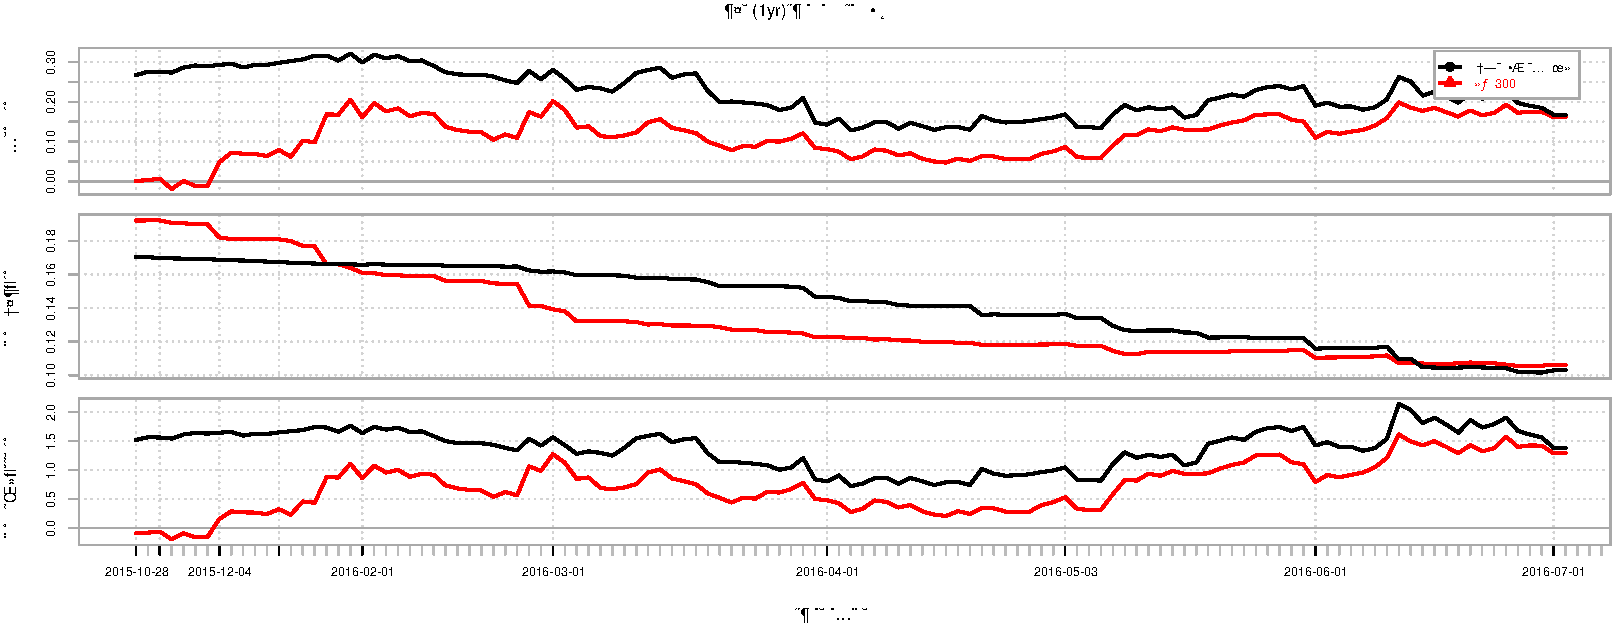
\includegraphics{hongliu-details_files/figure-latex/unnamed-chunk-5-1.pdf}

\section{风格分析}

\subsection{交易风格}

基于公开信息,我们对洪流的正在管理的圆信永丰双红利A的交易风格分析如下:

\begin{longtable}[]{@{}lcccccc@{}}
\toprule
日期 & 换手率 & 排名\% & 持有期 & 排名\% & 前十占比\% &
排名\%\tabularnewline
\midrule
\endhead
2015 Q2 & 819 & 12 & NA & 0 & 60 & 44\tabularnewline
2015 Q4 & 1439 & 27 & NA & 0 & 50 & 64\tabularnewline
2016 Q2 & 239 & 47 & 0.23 & 65 & 49 & 67\tabularnewline
2016 Q4 & 424 & 53 & 0.12 & 72 & 45 & 74\tabularnewline
\bottomrule
\end{longtable}

\begin{longtable}[]{@{}lccccrcrc@{}}
\toprule
日期 & 行业前5占比\% & 排名\% & 平均集中度 & 排名\% & PE & 排名\% & PB &
排名\%\tabularnewline
\midrule
\endhead
2015 Q2 & 95 & 58 & 0.22 & 56 & 20 & 86 & 3.5 & 84\tabularnewline
2015 Q4 & 86 & 89 & 0.33 & 37 & 33 & 69 & 3.5 & 75\tabularnewline
2016 Q2 & 98 & 45 & 0.26 & 35 & 27 & 66 & 5.0 & 31\tabularnewline
2016 Q4 & 94 & 61 & 0.32 & 26 & 21 & 64 & 2.7 & 53\tabularnewline
\bottomrule
\end{longtable}

换手率略高而持有期处于中间偏下。持股的平均PE和PB都在平均水平之下。从以上表格中可以看出
\emph{洪流,除了低的PB和PE暗示他的价值投资者身份外,在持股集中度,换手率等方面都是``中庸''型的}。

同样的对于圆信永丰优加生活进行交易风格分析,我们也发现了相似的情况。数据如下:

\begin{longtable}[]{@{}lcccccc@{}}
\toprule
日期 & 换手率 & 排名\% & 持有期 & 排名\% & 前十占比\% &
排名\%\tabularnewline
\midrule
\endhead
2015 Q4 & 876 & 39 & NA & 0 & 73 & 1\tabularnewline
2016 Q2 & 180 & 53 & 0.27 & 63 & 49 & 53\tabularnewline
2016 Q4 & 255 & 73 & 0.18 & 52 & 38 & 76\tabularnewline
\bottomrule
\end{longtable}

\begin{longtable}[]{@{}lccccrcrc@{}}
\toprule
日期 & 行业前5占比\% & 排名\% & 平均集中度 & 排名\% & PE & 排名\% & PB &
排名\%\tabularnewline
\midrule
\endhead
2015 Q4 & 91 & 57 & 0.27 & 52 & 42 & 61 & 3.6 & 78\tabularnewline
2016 Q2 & 96 & 48 & 0.12 & 60 & 33 & 58 & 4.3 & 49\tabularnewline
2016 Q4 & 84 & 91 & 0.12 & 58 & 23 & 75 & 3.2 & 50\tabularnewline
\bottomrule
\end{longtable}

需要进一步解释的是为什么2015
Q4显示的风格与其他时段不一致。这是因为基金刚刚创建,甚至仓位可能都还没有加满,一切都还在动态调整中。

\subsection{持仓风格}

基于净值数据,我们对洪流的持仓风格分析如下。

\subsubsection{圆信永丰双红利A}\label{a-1}

\begin{longtable}[]{@{}cccc@{}}
\caption{持仓风格权重分析(\%)}\tabularnewline
\toprule
大盘价值 & 小盘成长 & 债券财富指数 & 货币\tabularnewline
\midrule
\endfirsthead
\toprule
大盘价值 & 小盘成长 & 债券财富指数 & 货币\tabularnewline
\midrule
\endhead
6.9 & 66 & 20 & 7.3\tabularnewline
\bottomrule
\end{longtable}

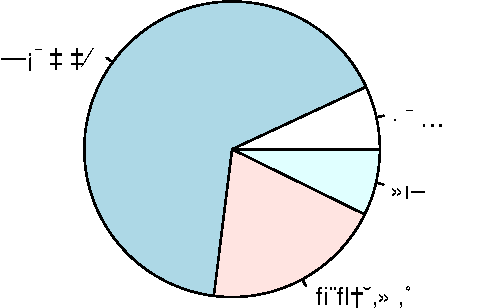
\includegraphics{hongliu-details_files/figure-latex/unnamed-chunk-8-1.pdf}

虽然我们的风格分析是基于净值数据的,但是经过比较持仓数据,结果还是相当准确的。尽管江湖传说作为徐京德的门徒,洪流应该是价值投资者,但事实是他应该是成长价值投资者\footnote{在此,我们讨论一下中国当前语境下的价值股和成长股投资。实际上投资这两种类型股票的投资这都应该是广义上的价值投资者,他们都是基于对于投资标的的价值判断做出的投资。区别是,价值股强调过去和当前的业绩显示出实实在在的投资价值,成长股则强调成长性,而且往往应为成长性有了一定的估值溢价。而这种基于未来不确定的成长性的估值溢价就为这类型的股票带来更多的不确定性和某种形式的周期性。因此投资这两类股票的价值投资者往往在风格上呈现足够的差异。久而久之,渐渐成为两个不同“流派”。所以成熟的投资者,不会拘泥与价值成长的区别,说白了,都是价值投资,都是在衡量价格与看得见的现在和看不见的未来之间匹配关系。不过,我们还是根据习惯,将他投资的两个属性合在一起表征他的投资风格。}。

\subsubsection{圆信永丰优加生活}\label{-1}

\begin{longtable}[]{@{}ccccc@{}}
\caption{持仓风格权重分析(\%)}\tabularnewline
\toprule
大盘价值 & 中盘成长 & 小盘价值 & 债券财富指数 & 货币\tabularnewline
\midrule
\endfirsthead
\toprule
大盘价值 & 中盘成长 & 小盘价值 & 债券财富指数 & 货币\tabularnewline
\midrule
\endhead
6.3 & 63 & 16 & 1.1 & 14\tabularnewline
\bottomrule
\end{longtable}

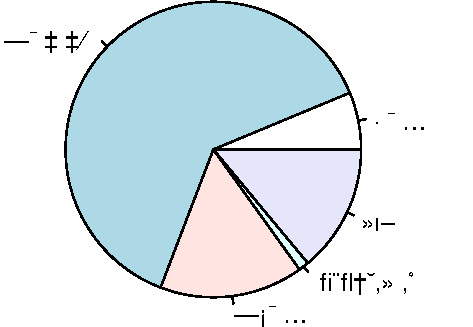
\includegraphics{hongliu-details_files/figure-latex/unnamed-chunk-9-1.pdf}

该基金是关注于``健康''和``生活''相关的主题型的基金。``健康''类别里头多有中盘成长股,``生活''相关常见价值股。出现这样的持股风格并不奇怪。这也表明,\emph{作为整个基金公司的投资总监,洪流能够和他的基金经理一起驾驭不同类型的投资风格。}
管理一只基金也许一个鲜明的风格就可以了,但是管理一家基金公司,一定要能够兼容并蓄,因为谁也不知道那棵树上能结果子。

\subsection{主动风格:积极}

以其管理的圆信永丰双红利A基金来看,该基金的平均主动管理活跃度为24\%。在其管理的同期,整个基金行业的同类型基金的主动管理活跃指数为27\%。
另一支基金圆信永丰优加生活平均主动管理活跃度为25\%。在其管理的同期,整个基金行业的同类型基金的主动管理活跃指数为27\%。
因此,\emph{对于洪流的管理风格可以定义为中庸的主动管理型}。

\section{能力评价}

\subsection{大类资产配置:几乎为零}

从下图可以看出,自从2014年11月以来,洪流在产品圆信永丰双红利A中将股票仓位控制在75-90\%之间,而另外一个产品圆信永丰优加生活股票仓位则也类似的在80\%-85\%之间变换。

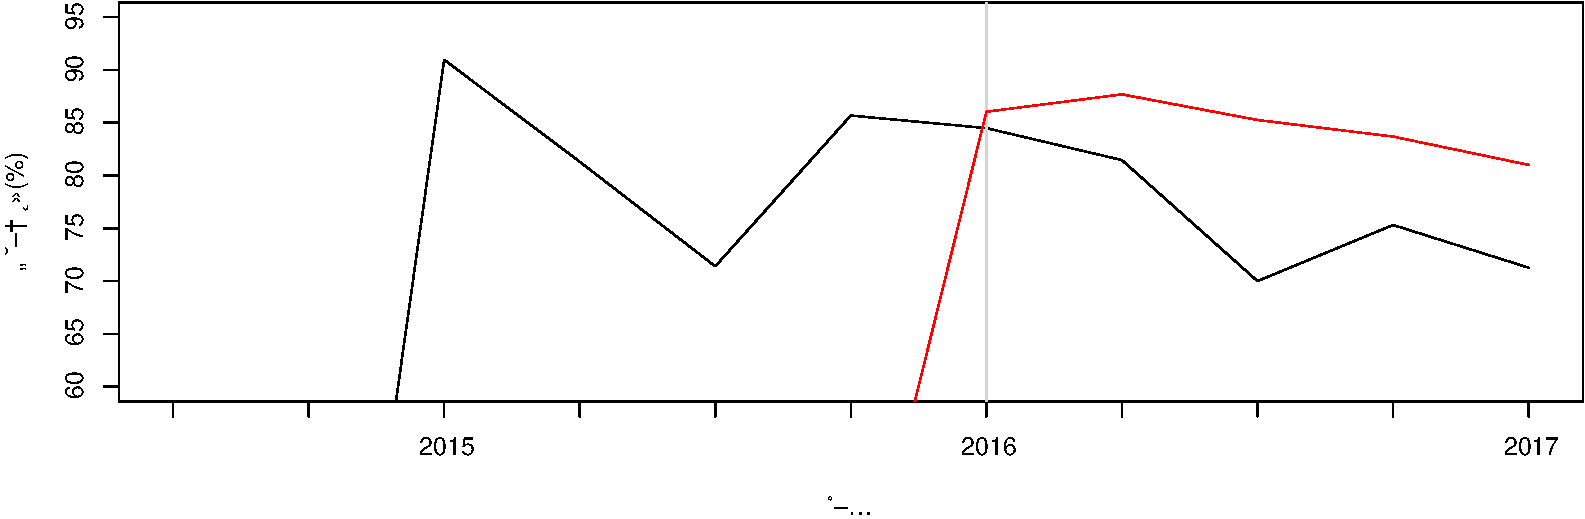
\includegraphics{hongliu-details_files/figure-latex/unnamed-chunk-11-1.pdf}

进一步的计算大类资产配置带来的超额收益。

\subsubsection{圆信永丰双红利A}\label{a-2}

\begin{longtable}[]{@{}lc@{}}
\caption{圆信永丰双红利A大类资产配置能力统计}\tabularnewline
\toprule
日期 & 大类资产配置超额贡献(\%)\tabularnewline
\midrule
\endfirsthead
\toprule
日期 & 大类资产配置超额贡献(\%)\tabularnewline
\midrule
\endhead
2015 Q1 & -3.20\tabularnewline
2015 Q2 & 1.21\tabularnewline
2015 Q3 & -2.04\tabularnewline
2015 Q4 & 1.01\tabularnewline
2016 Q1 & -2.28\tabularnewline
2016 Q2 & -0.28\tabularnewline
2016 Q3 & -0.10\tabularnewline
2016 Q4 & 0.43\tabularnewline
2017 Q1 & 0.26\tabularnewline
\bottomrule
\end{longtable}

\begin{longtable}[]{@{}cl@{}}
\toprule
平均超额贡献(\%) & 90\%置信区间\tabularnewline
\midrule
\endhead
-0.55 & \([-1.28,\infty)\)\tabularnewline
\bottomrule
\end{longtable}

统计显示,在圆信永丰双红利A这支基金的管理上,每季度平均取得 -0.55\%
的配置收益。因此洪流并没有显示出大类资产配置的能力。

\subsubsection{圆信永丰优加生活}\label{-2}

\begin{longtable}[]{@{}lc@{}}
\caption{圆信永丰双红利A大类资产配置能力统计}\tabularnewline
\toprule
日期 & 大类资产配置超额贡献(\%)\tabularnewline
\midrule
\endfirsthead
\toprule
日期 & 大类资产配置超额贡献(\%)\tabularnewline
\midrule
\endhead
2016 Q1 & 2.8671\tabularnewline
2016 Q2 & -0.1435\tabularnewline
2016 Q3 & -0.0071\tabularnewline
2016 Q4 & 0.4057\tabularnewline
2017 Q1 & 0.2272\tabularnewline
\bottomrule
\end{longtable}

\begin{longtable}[]{@{}cl@{}}
\toprule
平均超额贡献\% & 90\%置信区间\tabularnewline
\midrule
\endhead
0.67 & \([-0.18,\infty)\)\tabularnewline
\bottomrule
\end{longtable}

统计显示,在中欧潜力价值灵活配置混合这支基金的管理上,每季度平均取得
0.67\% 的配置收益,但是统计意义上不显著。

综上,结合仓位控制上的变化以及专项计算的大类资产配置对于收益的贡献。我们不得不说洪流,旗下基金管理中,没有表现出统计显著的大类资产配置的能力。他自己论述配置上的功夫时说道,``主要是根据牛熊判断控制仓位调整''。在我们的考察期内,牛熊变换发生了一次,几乎出乎所有人的判断,故而无所作为。
另一个重要的原因是他在基金产品设计的时候有明显的股票主题倾向(这从基金名称可以看出来),那么潜在的基金客户就是偏好于投资这类主题股票的投资者,配置是基金投资者需要考虑的问题,作为主题基金只需要在该主题范围内为投资者提供尽可能好的风险收益比就行了。从这个意义上说,未显示出来的大类资产配置能力不见得是洪流不具备,而是不需要而已。

\subsection{行业配置能力:较好}

既然基金产品的超额收益并非得益于大类资产的配置,那么比如来自与行业配置\footnote{我们使用的是证监会行业分类(一级)标准。}、选股以及择时的能力。需要提前指出的是,这三个能力在逻辑与实践中都不是相互独立的。好的投资标的往往也意味着好的投资时机,而好股票的挖掘与选择自然也带来了相应行业的配置偏好。但是这三种能力又在某种程度上可以区别开来,因为它们毕竟是在投资的不同决策层面和时点上的投资活动。我们认为:

\begin{longtable}[]{@{}lll@{}}
\toprule
行为 & 动机 & 度量方法\tabularnewline
\midrule
\endhead
行业配置 & smart beta & \(\sum(w_i-w_i^B)(r_i^B-r^B)\)\tabularnewline
择股 & 持续的alpha & \(\sum w_{i}(r_{i}^F-r_{i}^B)\)\tabularnewline
择时 & 动态的alpha & 未解释的差额部分\tabularnewline
\bottomrule
\end{longtable}

因为所获得数据精确程度的不同,我们计算的以上三个方面能力对于总超额收益的贡献比例可能是不精确的,读者应该更多的关注其相对值以及相关的统计推论。

\begin{longtable}[]{@{}lcc@{}}
\caption{圆信永丰双红利A行业配置能力}\tabularnewline
\toprule
日期 & 行业配置成功率\% & 行业配置贡献超额收益率\%\tabularnewline
\midrule
\endfirsthead
\toprule
日期 & 行业配置成功率\% & 行业配置贡献超额收益率\%\tabularnewline
\midrule
\endhead
2015 Q1 & 11.1 & 3.51\tabularnewline
2015 Q2 & 11.1 & 4.04\tabularnewline
2015 Q4 & 12.5 & 3.23\tabularnewline
2016 Q1 & 9.1 & -1.76\tabularnewline
2016 Q2 & -11.1 & 0.92\tabularnewline
2016 Q4 & 10.0 & 0.00\tabularnewline
2017 Q1 & 11.1 & 0.24\tabularnewline
\bottomrule
\end{longtable}

\begin{longtable}[]{@{}cl@{}}
\toprule
平均超额贡献\% & 90\%置信区间\tabularnewline
\midrule
\endhead
1.4 & \([0.27,\infty)\)\tabularnewline
\bottomrule
\end{longtable}

从统计结果可以看出,洪流在圆信永丰双红利A基金的管理上显示了一定的行业配置能力,平均超额表现为1.45\%每半年,年化5.95\%。

\begin{longtable}[]{@{}lcc@{}}
\caption{圆信永丰优加生活行业配置能力}\tabularnewline
\toprule
日期 & 行业配置成功率\% & 行业配置贡献超额收益率\%\tabularnewline
\midrule
\endfirsthead
\toprule
日期 & 行业配置成功率\% & 行业配置贡献超额收益率\%\tabularnewline
\midrule
\endhead
2016 Q1 & 11.1 & -0.47\tabularnewline
2016 Q2 & -10.0 & 0.64\tabularnewline
2016 Q4 & 8.3 & -0.38\tabularnewline
2017 Q1 & 9.1 & 0.14\tabularnewline
\bottomrule
\end{longtable}

\begin{longtable}[]{@{}cl@{}}
\toprule
平均超额贡献\% & 90\%置信区间\tabularnewline
\midrule
\endhead
-0.02 & \([-0.44,\infty)\)\tabularnewline
\bottomrule
\end{longtable}

从统计结果可以看出,洪流在圆信永丰优加生活基金的管理上没有显著的行业配置能力,平均超额表现为-0.02\%每半年,年化-0.06\%。这可能跟基金运营时间尚短有关系。

在洪流管理基金过程中,表现出一定的行业配置的能力,但是相应的不确定性大。

\subsection{择股能力:较强!}

公开渠道获得的持仓数据频率为每半年一次。我们依据此数据分析基金管理人的择股能力。当然,由于更新频率粗糙,读者有理由担心计算精度的问题。不过从另外一个角度看,我们所谓的择股能力是对照于择时能力而言获取相对持续的alpha的能力。这里的相对持续,完全可以根据我们研究的需要而定义。此处,定义半年为一个相对持续的alpha的标准,也是合情合理的。当前受制于数据不完整,此项能力分析最早只能回溯到2013年。

\begin{longtable}[]{@{}lcc@{}}
\caption{圆信永丰双红利A择股能力}\tabularnewline
\toprule
日期 & 行业择股成功率\% & 择股贡献超额收益率\%\tabularnewline
\midrule
\endfirsthead
\toprule
日期 & 行业择股成功率\% & 择股贡献超额收益率\%\tabularnewline
\midrule
\endhead
2015 Q1-2 & 11.1 & 15.38\tabularnewline
2015 Q3-4 & 10.0 & 7.24\tabularnewline
2016 Q1-2 & 9.1 & 10.54\tabularnewline
2016 Q3-4 & -9.1 & -3.84\tabularnewline
2017 Q1-2 & -9.1 & 12.52\tabularnewline
2017 Q3-4 & -33.3 & 0.34\tabularnewline
\bottomrule
\end{longtable}

\begin{longtable}[]{@{}cl@{}}
\toprule
平均超额贡献\% & 90\%置信区间\tabularnewline
\midrule
\endhead
7 & \([2.56,\infty)\)\tabularnewline
\bottomrule
\end{longtable}

从统计结果可以看出,洪流在圆信永丰双红利A基金的管理上显示了明显的择股能力------即她能够选择出在未来6个月的投资周期上回报好于对应行业指数表现的股票组合,而且择股能力贡献的平均超额表现高达7.03\%每半年,年化14.55\%。

\begin{longtable}[]{@{}lcc@{}}
\caption{圆信永丰优加生活择股能力}\tabularnewline
\toprule
日期 & 行业择股成功率\% & 择股贡献超额收益率\%\tabularnewline
\midrule
\endfirsthead
\toprule
日期 & 行业择股成功率\% & 择股贡献超额收益率\%\tabularnewline
\midrule
\endhead
2016 Q1-2 & 8.3 & 9.8\tabularnewline
2016 Q3-4 & -6.7 & -2.2\tabularnewline
2017 Q1-2 & -7.7 & 1.1\tabularnewline
\bottomrule
\end{longtable}

\begin{longtable}[]{@{}cl@{}}
\toprule
平均超额贡献\% & 90\%置信区间\tabularnewline
\midrule
\endhead
2.9 & \([-3.83,\infty)\)\tabularnewline
\bottomrule
\end{longtable}

从统计结果可以看出,洪流在圆信永丰优加生活基金的管理上显示了明显的择股能力------即她能够选择出在未来6个月的投资周期上回报好于对应行业指数表现的股票组合,而且择股能力贡献的平均超额表现高达2.91\%每半年,年化5.9\%。

\subsection{择时能力:不追求}

择时能力在本文的设定中包括以下方面:

\begin{itemize}
\tightlist
\item
  交易周期短于半年的动态alpha机会,如一些短期事件性投资机会、相对明确的业绩反转预期等。
\item
  上升通道中的止盈能力
\item
  下降通道中的止亏能力
\end{itemize}

所以择时能力并不总是能够带来正的超额收益,但是它能够确保落袋为安(止盈能力)或者保命再战(止亏能力),对于提高基金的风险收益比(如夏普率)是十分重要的。

\begin{longtable}[]{@{}lc@{}}
\caption{圆信永丰双红利A择时能力}\tabularnewline
\toprule
日期 & 择时能力贡献超额收益率\%\tabularnewline
\midrule
\endfirsthead
\toprule
日期 & 择时能力贡献超额收益率\%\tabularnewline
\midrule
\endhead
2015 Q1-2 & 72.1\tabularnewline
2015 Q3-4 & 9.3\tabularnewline
2016 Q1-2 & -1.7\tabularnewline
2016 Q3-4 & 5.6\tabularnewline
2017 Q1-2 & -6.3\tabularnewline
\bottomrule
\end{longtable}

\begin{longtable}[]{@{}cl@{}}
\toprule
平均超额贡献\% & 90\%置信区间\tabularnewline
\midrule
\endhead
16 & \([-6.19,\infty)\)\tabularnewline
\bottomrule
\end{longtable}

从上表中可以看出,洪流在圆信永丰双红利A基金的管理上显示了明显的择时能力,而且择时能力贡献的平均超额表现高达15.79\%每半年,年化34.08\%。但是,也要注意到择时能力的表现十分不稳定,主要贡献来着2015年上半年,这是因为基金创建于2014年底,当时建仓工作没有全部完成,而在2015年上半年进行了大幅度的建仓。我们的判定系统将这种行为判断为择时活动,因而给出了该期超高的择时能力,其实该部分收益当归结为择股能力。若排除这一项,实际上择时能力相当的弱。用他本人的话说``持有期多以年为单位,至少两季度'',在这样的风格下,当然不刻意追求短线获利的机会。

\begin{longtable}[]{@{}lc@{}}
\caption{圆信永丰优加生活择时能力}\tabularnewline
\toprule
日期 & 择时能力贡献超额收益率\%\tabularnewline
\midrule
\endfirsthead
\toprule
日期 & 择时能力贡献超额收益率\%\tabularnewline
\midrule
\endhead
2016 Q1-2 & 31.0\tabularnewline
2016 Q3-4 & 6.0\tabularnewline
2017 Q1-2 & 5.2\tabularnewline
\bottomrule
\end{longtable}

\begin{longtable}[]{@{}cl@{}}
\toprule
平均超额贡献\% & 90\%置信区间\tabularnewline
\midrule
\endhead
14 & \([-1.90,\infty)\)\tabularnewline
\bottomrule
\end{longtable}

从上表中可以看出,洪流在圆信永丰优加生活基金的管理上显示了明显的择时能力,而且择时能力贡献的平均超额表现为14.07\%每半年,年化30.12\%。同样的道理,该基金创建与2015年末,所以2016上半年的择时能力中有很大一部分应该归属于择股能力。尽管如此,他依旧在其后的表现中展现出了一定的择时能力。当然,考虑到圆信基金的组织架构,洪流的时间安排,我们更倾向与将该部分的表现归功于另外以为共同管理该基金的范妍女士。

综上,我们认为洪流作为一名偏好长期投资的投资者和圆信基金的投资负责人,没有动机与时间去关注短时alpha机会的。

\section{投资方法体系}

\subsection{股市中的绝对收益}

利用动态投资策略,在股市中获取绝对收益:

\begin{itemize}
\item
  用1-3个月的时间,低于20\%的股票仓位,利用无风险收益和股票市场中确定性比较的机会累计初始安全垫
\item
  当净值\(\geq 1.05\),增加仓位,同时提高安全垫的标准(即提高止损的标准,如净值1.03)
\end{itemize}

如此,实现了累计收益阶梯式的增长并有效的控制回撤,虽然不见得获得了最大的投资收益,但是收益风险比一定是靓丽的。

\subsection{投资研究方法}

\begin{itemize}

\item 战略判断(实际是中观分析),包括:
\begin{enumerate}
\item 行业周期:判断行业是否景气
\item 企业家精神:判断核心管理者的素质和团队战略管理方面的质量
\item 当前赛道的判断:长期的毛利水平,是否适应新的发展等
\end{enumerate}
\item 核心股票池跟踪(100个左右),要求
\begin{enumerate}
\item 持续的可预见的盈利增长
\item 拥有完整的数据链以支持研究判断
\item 月报、季报细致比较,动态跟踪风险收益比。
\end{enumerate}
\end{itemize}

\section{评价}

洪流是资深的投资人。他具备数学本科的背景,工作经历上提供了完整的管理能力、资产配置能力与资管能力的训练,同时形成了一个强大的朋友圈,这些都成为他投资上不可或缺的资源。我们基于公开信息,进行深度的科学分析,结合与其面对面的交流,做出如下评判:

\begin{enumerate}
\def\labelenumi{\arabic{enumi}.}
\tightlist
\item
  洪流有偏好长期价值,但是同时能够驾驭多种不同风格的基金管理者;
\item
  洪流有着成熟的行业分析方法和经验,能够从行业轮动中获取配置的机会,因而具备较好的行业配置的能力;
\item
  洪流具备了足够的经历去理解分析企业管理层,从而能够结合行业分析选取出好的投资标的,因此具备较强的择股能力;
\item
  当前的工作需要并没有挑战他的大类资产配置能力,我们只能说,洪流没有展示出大类资产配置的能力。
\end{enumerate}

因此,洪流是有着丰富的经历和阅历,具备深度行业分析与配置能力,较强的择股能力的基金管理者;同时他也具备强大的气质和管理经验,是一位成熟的基金经理的经理。

\end{document}
